\chapter{Shortest paths}

\index{shortest path}

Finding a shortest path between two nodes
of a graph
is an important problem that has many
practical applications.
For example, a natural problem related to a road network
is to calculate the shortest possible length of a route
between two cities, given the lengths of the roads.

In an unweighted graph, the length of a path equals
the number of its edges, and we can
simply use breadth-first search to find
a shortest path.
However, in this chapter we focus on
weighted graphs
where more sophisticated algorithms
are needed
for finding shortest paths.

\section{Bellman–Ford algorithm}

\index{Bellman–Ford algorithm}

The \key{Bellman–Ford algorithm}\footnote{The algorithm is named after
R. E. Bellman and L. R. Ford who published it independently
in 1958 and 1956, respectively \cite{bel58,for56a}.} finds
shortest paths from a starting node to all
nodes of the graph.
The algorithm can process all kinds of graphs,
provided that the graph does not contain a
cycle with negative length.
If the graph contains a negative cycle,
the algorithm can detect this.

The algorithm keeps track of distances
from the starting node to all nodes of the graph.
Initially, the distance to the starting node is 0
and the distance to all other nodes in infinite.
The algorithm reduces the distances by finding
edges that shorten the paths until it is not
possible to reduce any distance.

\subsubsection{Example}

Let us consider how the Bellman–Ford algorithm
works in the following graph:
\begin{center}
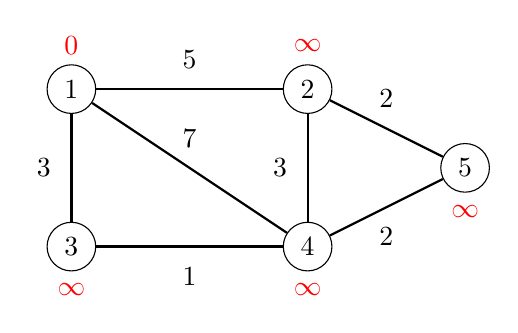
\begin{tikzpicture}
\node[draw, circle] (1) at (1,3) {1};
\node[draw, circle] (2) at (4,3) {2};
\node[draw, circle] (3) at (1,1) {3};
\node[draw, circle] (4) at (4,1) {4};
\node[draw, circle] (5) at (6,2) {5};
\node[color=red] at (1,3+0.55) {$0$};
\node[color=red] at (4,3+0.55) {$\infty$};
\node[color=red] at (1,1-0.55) {$\infty$};
\node[color=red] at (4,1-0.55) {$\infty$};
\node[color=red] at (6,2-0.55) {$\infty$};
\path[draw,thick,-] (1) -- node[font=\small,label=above:5] {} (2);
\path[draw,thick,-] (1) -- node[font=\small,label=left:3] {} (3);
\path[draw,thick,-] (3) -- node[font=\small,label=below:1] {} (4);
\path[draw,thick,-] (2) -- node[font=\small,label=left:3] {} (4);
\path[draw,thick,-] (2) -- node[font=\small,label=above:2] {} (5);
\path[draw,thick,-] (4) -- node[font=\small,label=below:2] {} (5);
\path[draw,thick,-] (1) -- node[font=\small,label=above:7] {} (4);
\end{tikzpicture}
\end{center}
Each node of the graph is assigned a distance.
Initially, the distance to the starting node is 0,
and the distance to all other nodes is infinite.

The algorithm searches for edges that reduce distances.
First, all edges from node 1 reduce distances:
\begin{center}
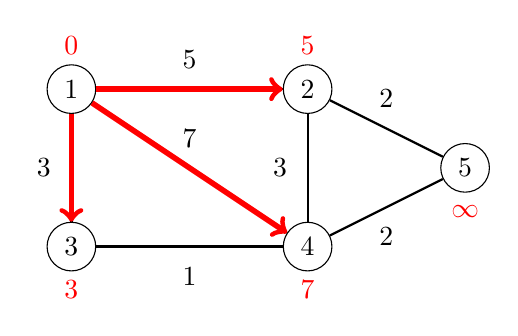
\begin{tikzpicture}
\node[draw, circle] (1) at (1,3) {1};
\node[draw, circle] (2) at (4,3) {2};
\node[draw, circle] (3) at (1,1) {3};
\node[draw, circle] (4) at (4,1) {4};
\node[draw, circle] (5) at (6,2) {5};
\node[color=red] at (1,3+0.55) {$0$};
\node[color=red] at (4,3+0.55) {$5$};
\node[color=red] at (1,1-0.55) {$3$};
\node[color=red] at (4,1-0.55) {$7$};
\node[color=red] at (6,2-0.55) {$\infty$};
\path[draw,thick,-] (1) -- node[font=\small,label=above:5] {} (2);
\path[draw,thick,-] (1) -- node[font=\small,label=left:3] {} (3);
\path[draw,thick,-] (3) -- node[font=\small,label=below:1] {} (4);
\path[draw,thick,-] (2) -- node[font=\small,label=left:3] {} (4);
\path[draw,thick,-] (2) -- node[font=\small,label=above:2] {} (5);
\path[draw,thick,-] (4) -- node[font=\small,label=below:2] {} (5);
\path[draw,thick,-] (1) -- node[font=\small,label=above:7] {} (4);

\path[draw=red,thick,->,line width=2pt] (1) -- (2);
\path[draw=red,thick,->,line width=2pt] (1) -- (3);
\path[draw=red,thick,->,line width=2pt] (1) -- (4);
\end{tikzpicture}
\end{center}
After this, edges
$2 \rightarrow 5$ and $3 \rightarrow 4$
reduce distances:
\begin{center}
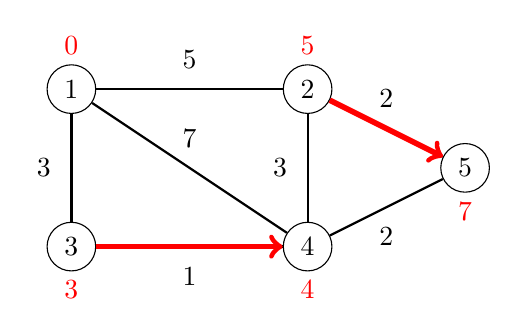
\begin{tikzpicture}
\node[draw, circle] (1) at (1,3) {1};
\node[draw, circle] (2) at (4,3) {2};
\node[draw, circle] (3) at (1,1) {3};
\node[draw, circle] (4) at (4,1) {4};
\node[draw, circle] (5) at (6,2) {5};
\node[color=red] at (1,3+0.55) {$0$};
\node[color=red] at (4,3+0.55) {$5$};
\node[color=red] at (1,1-0.55) {$3$};
\node[color=red] at (4,1-0.55) {$4$};
\node[color=red] at (6,2-0.55) {$7$};
\path[draw,thick,-] (1) -- node[font=\small,label=above:5] {} (2);
\path[draw,thick,-] (1) -- node[font=\small,label=left:3] {} (3);
\path[draw,thick,-] (3) -- node[font=\small,label=below:1] {} (4);
\path[draw,thick,-] (2) -- node[font=\small,label=left:3] {} (4);
\path[draw,thick,-] (2) -- node[font=\small,label=above:2] {} (5);
\path[draw,thick,-] (4) -- node[font=\small,label=below:2] {} (5);
\path[draw,thick,-] (1) -- node[font=\small,label=above:7] {} (4);

\path[draw=red,thick,->,line width=2pt] (2) -- (5);
\path[draw=red,thick,->,line width=2pt] (3) -- (4);
\end{tikzpicture}
\end{center}
Finally, there is one more change:
\begin{center}
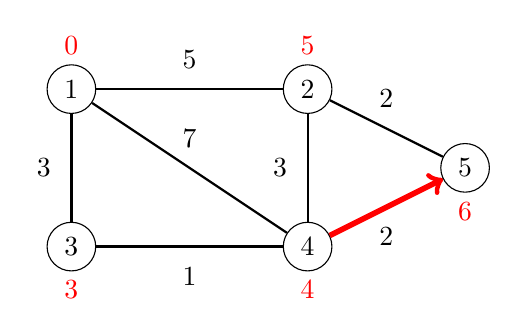
\begin{tikzpicture}
\node[draw, circle] (1) at (1,3) {1};
\node[draw, circle] (2) at (4,3) {2};
\node[draw, circle] (3) at (1,1) {3};
\node[draw, circle] (4) at (4,1) {4};
\node[draw, circle] (5) at (6,2) {5};
\node[color=red] at (1,3+0.55) {$0$};
\node[color=red] at (4,3+0.55) {$5$};
\node[color=red] at (1,1-0.55) {$3$};
\node[color=red] at (4,1-0.55) {$4$};
\node[color=red] at (6,2-0.55) {$6$};
\path[draw,thick,-] (1) -- node[font=\small,label=above:5] {} (2);
\path[draw,thick,-] (1) -- node[font=\small,label=left:3] {} (3);
\path[draw,thick,-] (3) -- node[font=\small,label=below:1] {} (4);
\path[draw,thick,-] (2) -- node[font=\small,label=left:3] {} (4);
\path[draw,thick,-] (2) -- node[font=\small,label=above:2] {} (5);
\path[draw,thick,-] (4) -- node[font=\small,label=below:2] {} (5);
\path[draw,thick,-] (1) -- node[font=\small,label=above:7] {} (4);

\path[draw=red,thick,->,line width=2pt] (4) -- (5);
\end{tikzpicture}
\end{center}

After this, no edge can reduce any distance.
This means that the distances are final,
and we have successfully
calculated the shortest distances
from the starting node to all nodes of the graph.

For example, the shortest distance 3
from node 1 to node 5 corresponds to
the following path:

\begin{center}
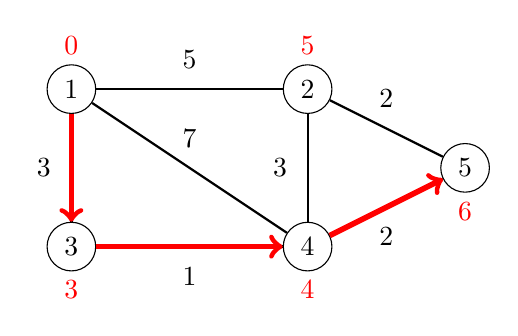
\begin{tikzpicture}
\node[draw, circle] (1) at (1,3) {1};
\node[draw, circle] (2) at (4,3) {2};
\node[draw, circle] (3) at (1,1) {3};
\node[draw, circle] (4) at (4,1) {4};
\node[draw, circle] (5) at (6,2) {5};
\node[color=red] at (1,3+0.55) {$0$};
\node[color=red] at (4,3+0.55) {$5$};
\node[color=red] at (1,1-0.55) {$3$};
\node[color=red] at (4,1-0.55) {$4$};
\node[color=red] at (6,2-0.55) {$6$};
\path[draw,thick,-] (1) -- node[font=\small,label=above:5] {} (2);
\path[draw,thick,-] (1) -- node[font=\small,label=left:3] {} (3);
\path[draw,thick,-] (3) -- node[font=\small,label=below:1] {} (4);
\path[draw,thick,-] (2) -- node[font=\small,label=left:3] {} (4);
\path[draw,thick,-] (2) -- node[font=\small,label=above:2] {} (5);
\path[draw,thick,-] (4) -- node[font=\small,label=below:2] {} (5);
\path[draw,thick,-] (1) -- node[font=\small,label=above:7] {} (4);

\path[draw=red,thick,->,line width=2pt] (1) -- (3);
\path[draw=red,thick,->,line width=2pt] (3) -- (4);
\path[draw=red,thick,->,line width=2pt] (4) -- (5);
\end{tikzpicture}
\end{center}

\subsubsection{Implementation}

The following implementation of the
Bellman–Ford algorithm determines the shortest distances
from a node $x$ to all nodes of the graph.
The code assumes that the graph is stored
as an edge list \texttt{edges}
that consists of tuples of the form $(a,b,w)$,
meaning that there is an edge from node $a$ to node $b$
with weight $w$.

The algorithm consists of $n-1$ rounds,
and on each round the algorithm goes through
all edges of the graph and tries to
reduce the distances.
The algorithm constructs an array \texttt{distance}
that will contain the distances from $x$
to all nodes of the graph.
The constant \texttt{INF} denotes an infinite distance.

\begin{lstlisting}
for (int i = 1; i <= n; i++) distance[i] = INF;
distance[x] = 0;
for (int i = 1; i <= n-1; i++) {
    for (auto e : edges) {
        int a, b, w;
        tie(a, b, w) = e;
        distance[b] = min(distance[b], distance[a]+w);
    }
}
\end{lstlisting}

The time complexity of the algorithm is $O(nm)$,
because the algorithm consists of $n-1$ rounds and
iterates through all $m$ edges during a round.
If there are no negative cycles in the graph,
all distances are final after $n-1$ rounds,
because each shortest path can contain at most $n-1$ edges.

In practice, the final distances can usually
be found faster than in $n-1$ rounds.
Thus, a possible way to make the algorithm more efficient
is to stop the algorithm if no distance
can be reduced during a round.

\subsubsection{Negative cycles}

\index{negative cycle}

The Bellman–Ford algorithm can also be used to
check if the graph contains a cycle with negative length.
For example, the graph

\begin{center}
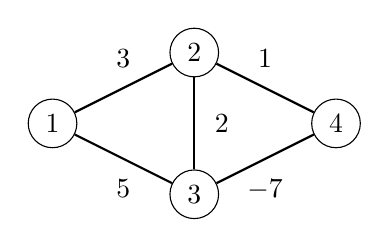
\begin{tikzpicture}[scale=0.9]
\node[draw, circle] (1) at (0,0) {$1$};
\node[draw, circle] (2) at (2,1) {$2$};
\node[draw, circle] (3) at (2,-1) {$3$};
\node[draw, circle] (4) at (4,0) {$4$};

\path[draw,thick,-] (1) -- node[font=\small,label=above:$3$] {} (2);
\path[draw,thick,-] (2) -- node[font=\small,label=above:$1$] {} (4);
\path[draw,thick,-] (1) -- node[font=\small,label=below:$5$] {} (3);
\path[draw,thick,-] (3) -- node[font=\small,label=below:$-7$] {} (4);
\path[draw,thick,-] (2) -- node[font=\small,label=right:$2$] {} (3);
\end{tikzpicture}
\end{center}
\noindent
contains a negative cycle
$2 \rightarrow 3 \rightarrow 4 \rightarrow 2$
with length $-4$.

If the graph contains a negative cycle,
we can shorten infinitely many times
any path that contains the cycle by repeating the cycle
again and again.
Thus, the concept of a shortest path
is not meaningful in this situation.

A negative cycle can be detected
using the Bellman–Ford algorithm by
running the algorithm for $n$ rounds.
If the last round reduces any distance,
the graph contains a negative cycle.
Note that this algorithm can be used to
search for
a negative cycle in the whole graph
regardless of the starting node.

\subsubsection{SPFA algorithm}

\index{SPFA algorithm}

The \key{SPFA algorithm} (''Shortest Path Faster Algorithm'') \cite{fan94}
is a variant of the Bellman–Ford algorithm,
that is often more efficient than the original algorithm.
The SPFA algorithm does not go through all the edges on each round,
but instead, it chooses the edges to be examined
in a more intelligent way.

The algorithm maintains a queue of nodes that might
be used for reducing the distances.
First, the algorithm adds the starting node $x$
to the queue.
Then, the algorithm always processes the
first node in the queue, and when an edge
$a \rightarrow b$ reduces a distance,
node $b$ is added to the queue.
% 
% The following implementation uses a 
% \texttt{queue} \texttt{q}.
% In addition, an array \texttt{inqueue} indicates
% if a node is already in the queue,
% in which case the algorithm does not add
% the node to the queue again.
% 
% \begin{lstlisting}
% for (int i = 1; i <= n; i++) distance[i] = INF;
% distance[x] = 0;
% q.push(x);
% while (!q.empty()) {
%     int a = q.front(); q.pop();
%     inqueue[a] = false;
%     for (auto b : v[a]) {
%         if (distance[a]+b.second < distance[b.first]) {
%             distance[b.first] = distance[a]+b.second;
%             if (!inqueue[b]) {q.push(b); inqueue[b] = true;}
%         }
%     }
% }
% \end{lstlisting}

The efficiency of the SPFA algorithm depends
on the structure of the graph:
the algorithm is often efficient,
but its worst case time complexity is still
$O(nm)$ and it is possible to create inputs
that make the algorithm as slow as the
original Bellman–Ford algorithm.

\section{Dijkstra's algorithm}

\index{Dijkstra's algorithm}

\key{Dijkstra's algorithm}\footnote{E. W. Dijkstra published the algorithm in 1959 \cite{dij59};
however, his original paper does not mention how to implement the algorithm efficiently.}
finds shortest
paths from the starting node to all nodes of the graph,
like the Bellman–Ford algorithm.
The benefit of Dijsktra's algorithm is that
it is more efficient and can be used for
processing large graphs.
However, the algorithm requires that there
are no negative weight edges in the graph.

Like the Bellman–Ford algorithm,
Dijkstra's algorithm maintains distances
to the nodes and reduces them during the search.
Dijkstra's algorithm is efficient, because
it only processes
each edge in the graph once, using the fact
that there are no negative edges.

\subsubsection{Example}

Let us consider how Dijkstra's algorithm
works in the following graph when the
starting node is node 1:
\begin{center}
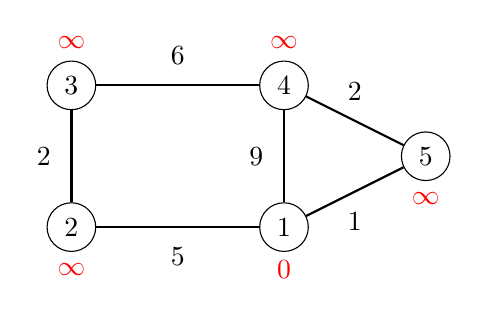
\begin{tikzpicture}[scale=0.9]
\node[draw, circle] (1) at (1,3) {3};
\node[draw, circle] (2) at (4,3) {4};
\node[draw, circle] (3) at (1,1) {2};
\node[draw, circle] (4) at (4,1) {1};
\node[draw, circle] (5) at (6,2) {5};

\node[color=red] at (1,3+0.6) {$\infty$};
\node[color=red] at (4,3+0.6) {$\infty$};
\node[color=red] at (1,1-0.6) {$\infty$};
\node[color=red] at (4,1-0.6) {$0$};
\node[color=red] at (6,2-0.6) {$\infty$};

\path[draw,thick,-] (1) -- node[font=\small,label=above:6] {} (2);
\path[draw,thick,-] (1) -- node[font=\small,label=left:2] {} (3);
\path[draw,thick,-] (3) -- node[font=\small,label=below:5] {} (4);
\path[draw,thick,-] (2) -- node[font=\small,label=left:9] {} (4);
\path[draw,thick,-] (2) -- node[font=\small,label=above:2] {} (5);
\path[draw,thick,-] (4) -- node[font=\small,label=below:1] {} (5);
\end{tikzpicture}
\end{center}
Like in the Bellman–Ford algorithm,
initially the distance to the starting node is 0
and the distance to all other nodes is infinite.

At each step, Dijkstra's algorithm selects a node
that has not been processed yet and whose distance
is as small as possible.
The first such node is node 1 with distance 0.

When a node is selected, the algorithm
goes through all edges that start at the node
and reduces the distances using them:
\begin{center}
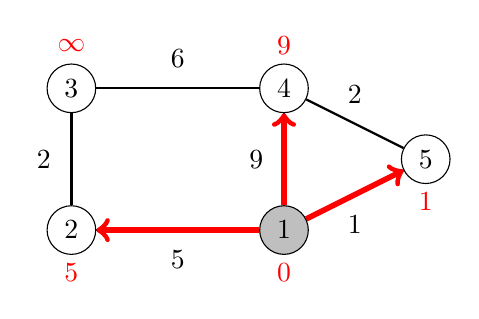
\begin{tikzpicture}[scale=0.9]
\node[draw, circle] (1) at (1,3) {3};
\node[draw, circle] (2) at (4,3) {4};
\node[draw, circle] (3) at (1,1) {2};
\node[draw, circle, fill=lightgray] (4) at (4,1) {1};
\node[draw, circle] (5) at (6,2) {5};

\node[color=red] at (1,3+0.6) {$\infty$};
\node[color=red] at (4,3+0.6) {$9$};
\node[color=red] at (1,1-0.6) {$5$};
\node[color=red] at (4,1-0.6) {$0$};
\node[color=red] at (6,2-0.6) {$1$};

\path[draw,thick,-] (1) -- node[font=\small,label=above:6] {} (2);
\path[draw,thick,-] (1) -- node[font=\small,label=left:2] {} (3);
\path[draw,thick,-] (3) -- node[font=\small,label=below:5] {} (4);
\path[draw,thick,-] (2) -- node[font=\small,label=left:9] {} (4);
\path[draw,thick,-] (2) -- node[font=\small,label=above:2] {} (5);
\path[draw,thick,-] (4) -- node[font=\small,label=below:1] {} (5);

\path[draw=red,thick,->,line width=2pt] (4) -- (2);
\path[draw=red,thick,->,line width=2pt] (4) -- (3);
\path[draw=red,thick,->,line width=2pt] (4) -- (5);
\end{tikzpicture}
\end{center}
In this case,
the edges from node 1 reduced the distances of
nodes 2, 4 and 5, whose distances are now 5, 9 and 1.

The next node to be processed is node 5 with distance 1.
This reduces the distance to node 4 from 9 to 3:
\begin{center}
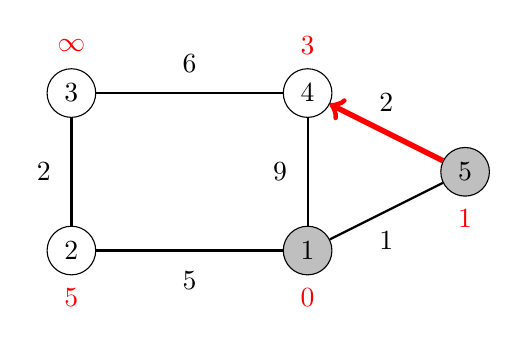
\begin{tikzpicture}
\node[draw, circle] (1) at (1,3) {3};
\node[draw, circle] (2) at (4,3) {4};
\node[draw, circle] (3) at (1,1) {2};
\node[draw, circle, fill=lightgray] (4) at (4,1) {1};
\node[draw, circle, fill=lightgray] (5) at (6,2) {5};

\node[color=red] at (1,3+0.6) {$\infty$};
\node[color=red] at (4,3+0.6) {$3$};
\node[color=red] at (1,1-0.6) {$5$};
\node[color=red] at (4,1-0.6) {$0$};
\node[color=red] at (6,2-0.6) {$1$};

\path[draw,thick,-] (1) -- node[font=\small,label=above:6] {} (2);
\path[draw,thick,-] (1) -- node[font=\small,label=left:2] {} (3);
\path[draw,thick,-] (3) -- node[font=\small,label=below:5] {} (4);
\path[draw,thick,-] (2) -- node[font=\small,label=left:9] {} (4);
\path[draw,thick,-] (2) -- node[font=\small,label=above:2] {} (5);
\path[draw,thick,-] (4) -- node[font=\small,label=below:1] {} (5);

\path[draw=red,thick,->,line width=2pt] (5) -- (2);
\end{tikzpicture}
\end{center}
After this, the next node is node 4, which reduces
the distance to node 3 to 9:
\begin{center}
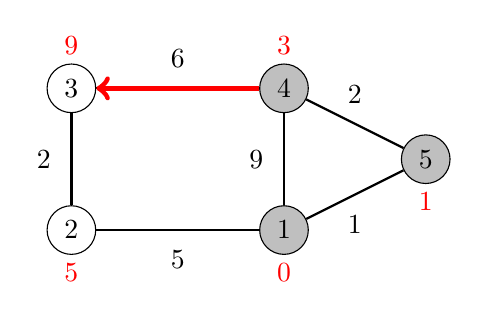
\begin{tikzpicture}[scale=0.9]
\node[draw, circle] (1) at (1,3) {3};
\node[draw, circle, fill=lightgray] (2) at (4,3) {4};
\node[draw, circle] (3) at (1,1) {2};
\node[draw, circle, fill=lightgray] (4) at (4,1) {1};
\node[draw, circle, fill=lightgray] (5) at (6,2) {5};

\node[color=red] at (1,3+0.6) {$9$};
\node[color=red] at (4,3+0.6) {$3$};
\node[color=red] at (1,1-0.6) {$5$};
\node[color=red] at (4,1-0.6) {$0$};
\node[color=red] at (6,2-0.6) {$1$};

\path[draw,thick,-] (1) -- node[font=\small,label=above:6] {} (2);
\path[draw,thick,-] (1) -- node[font=\small,label=left:2] {} (3);
\path[draw,thick,-] (3) -- node[font=\small,label=below:5] {} (4);
\path[draw,thick,-] (2) -- node[font=\small,label=left:9] {} (4);
\path[draw,thick,-] (2) -- node[font=\small,label=above:2] {} (5);
\path[draw,thick,-] (4) -- node[font=\small,label=below:1] {} (5);

\path[draw=red,thick,->,line width=2pt] (2) -- (1);
\end{tikzpicture}
\end{center}

A remarkable property in Dijkstra's algorithm is that
whenever a node is selected, its distance is final.
For example, at this point of the algorithm,
the distances 0, 1 and 3 are the final distances
to nodes 1, 5 and 4.

After this, the algorithm processes the two
remaining nodes, and the final distances are as follows:

\begin{center}
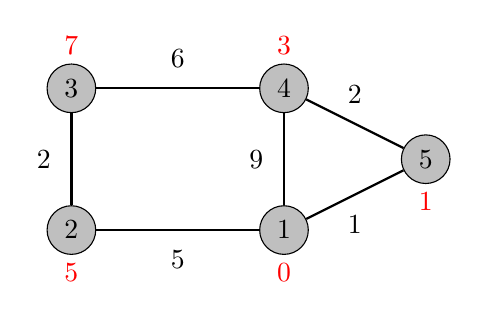
\begin{tikzpicture}[scale=0.9]
\node[draw, circle, fill=lightgray] (1) at (1,3) {3};
\node[draw, circle, fill=lightgray] (2) at (4,3) {4};
\node[draw, circle, fill=lightgray] (3) at (1,1) {2};
\node[draw, circle, fill=lightgray] (4) at (4,1) {1};
\node[draw, circle, fill=lightgray] (5) at (6,2) {5};

\node[color=red] at (1,3+0.6) {$7$};
\node[color=red] at (4,3+0.6) {$3$};
\node[color=red] at (1,1-0.6) {$5$};
\node[color=red] at (4,1-0.6) {$0$};
\node[color=red] at (6,2-0.6) {$1$};

\path[draw,thick,-] (1) -- node[font=\small,label=above:6] {} (2);
\path[draw,thick,-] (1) -- node[font=\small,label=left:2] {} (3);
\path[draw,thick,-] (3) -- node[font=\small,label=below:5] {} (4);
\path[draw,thick,-] (2) -- node[font=\small,label=left:9] {} (4);
\path[draw,thick,-] (2) -- node[font=\small,label=above:2] {} (5);
\path[draw,thick,-] (4) -- node[font=\small,label=below:1] {} (5);
\end{tikzpicture}
\end{center}

\subsubsection{Negative edges}

The efficiency of Dijkstra's algorithm is
based on the fact that the graph does not
contain negative edges.
If there is a negative edge,
the algorithm may give incorrect results.
As an example, consider the following graph:

\begin{center}
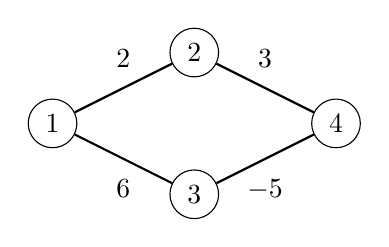
\begin{tikzpicture}[scale=0.9]
\node[draw, circle] (1) at (0,0) {$1$};
\node[draw, circle] (2) at (2,1) {$2$};
\node[draw, circle] (3) at (2,-1) {$3$};
\node[draw, circle] (4) at (4,0) {$4$};

\path[draw,thick,-] (1) -- node[font=\small,label=above:2] {} (2);
\path[draw,thick,-] (2) -- node[font=\small,label=above:3] {} (4);
\path[draw,thick,-] (1) -- node[font=\small,label=below:6] {} (3);
\path[draw,thick,-] (3) -- node[font=\small,label=below:$-5$] {} (4);
\end{tikzpicture}
\end{center}
\noindent
The shortest path from node 1 to node 4 is
$1 \rightarrow 3 \rightarrow 4$
and its length is 1.
However, Dijkstra's algorithm
finds the path $1 \rightarrow 2 \rightarrow 4$
by following the minimum weight edges.
The algorithm does not take into account that
on the other path, the weight $-5$
compensates the previous large weight $6$.

\subsubsection{Implementation}

The following implementation of Dijkstra's algorithm
calculates the minimum distances from a node $x$
to other nodes of the graph.
The graph is stored as adjacency lists
so that \texttt{adj[$a$]} contains a pair $(b,w)$
always when there is an edge from node $a$ to node $b$
with weight $w$.

An efficient implementation of Dijkstra's algorithm
requires that it is possible to efficiently find the
minimum distance node that has not been processed.
An appropriate data structure for this is a priority queue
that contains the nodes ordered by their distances.
Using a priority queue, the next node to be processed
can be retrieved in logarithmic time.

In the following code, the priority queue
\texttt{q} contains pairs of the form $(-d,x)$,
meaning that the current distance to node $x$ is $d$.
The array $\texttt{distance}$ contains the distance to
each node, and the array $\texttt{processed}$ indicates
whether a node has been processed.
Initially the distance is $0$ to $x$ and $\infty$ to all other nodes.

\begin{lstlisting}
for (int i = 1; i <= n; i++) distance[i] = INF;
distance[x] = 0;
q.push({0,x});
while (!q.empty()) {
    int a = q.top().second; q.pop();
    if (processed[a]) continue;
    processed[a] = true;
    for (auto u : adj[a]) {
        int b = u.first, w = u.second;
        if (distance[a]+w < distance[b]) {
            distance[b] = distance[a]+w;
            q.push({-distance[b],b});
        }
    }
}
\end{lstlisting}

Note that the priority queue contains \emph{negative}
distances to nodes.
The reason for this is that the
default version of the C++ priority queue finds maximum
elements, while we want to find minimum elements.
By using negative distances,
we can directly use the default priority queue\footnote{Of
course, we could also declare the priority queue as in Chapter 4.5
and use positive distances, but the implementation would be a bit longer.}.
Also note that there may be several instances of the same
node in the priority queue; however, only the instance with the
minimum distance will be processed.

The time complexity of the above implementation is
$O(n+m \log m)$, because the algorithm goes through
all nodes of the graph and adds for each edge
at most one distance to the priority queue.

\section{Floyd–Warshall algorithm}

\index{Floyd–Warshall algorithm}

The \key{Floyd–Warshall algorithm}\footnote{The algorithm
is named after R. W. Floyd and S. Warshall
who published it independently in 1962 \cite{flo62,war62}.}
provides an alternative way to approach the problem
of finding shortest paths.
Unlike the other algorithms of this chapter,
it finds all shortest paths between the nodes
in a single run.

The algorithm maintains a two-dimensional array
that contains distances between the nodes.
First, distances are calculated only using
direct edges between the nodes,
and after this, the algorithm reduces distances
by using intermediate nodes in paths.

\subsubsection{Example}

Let us consider how the Floyd–Warshall algorithm
works in the following graph:

\begin{center}
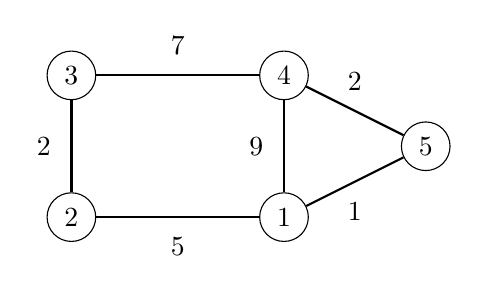
\begin{tikzpicture}[scale=0.9]
\node[draw, circle] (1) at (1,3) {$3$};
\node[draw, circle] (2) at (4,3) {$4$};
\node[draw, circle] (3) at (1,1) {$2$};
\node[draw, circle] (4) at (4,1) {$1$};
\node[draw, circle] (5) at (6,2) {$5$};

\path[draw,thick,-] (1) -- node[font=\small,label=above:7] {} (2);
\path[draw,thick,-] (1) -- node[font=\small,label=left:2] {} (3);
\path[draw,thick,-] (3) -- node[font=\small,label=below:5] {} (4);
\path[draw,thick,-] (2) -- node[font=\small,label=left:9] {} (4);
\path[draw,thick,-] (2) -- node[font=\small,label=above:2] {} (5);
\path[draw,thick,-] (4) -- node[font=\small,label=below:1] {} (5);
\end{tikzpicture}
\end{center}

Initially, the distance from each node to itself is $0$,
and the distance between nodes $a$ and $b$ is $x$
if there is an edge between nodes $a$ and $b$ with weight $x$.
All other distances are infinite.

In this graph, the initial array is as follows:
\begin{center}
\begin{tabular}{r|rrrrr}
 & 1 & 2 & 3 & 4 & 5 \\
\hline
1 & 0 & 5 & $\infty$ & 9 & 1 \\
2 & 5 & 0 & 2 & $\infty$ & $\infty$ \\
3 & $\infty$ & 2 & 0 & 7 & $\infty$ \\
4 & 9 & $\infty$ & 7 & 0 & 2 \\
5 & 1 & $\infty$ & $\infty$ & 2 & 0 \\
\end{tabular}
\end{center}
\vspace{10pt}
The algorithm consists of consecutive rounds.
On each round, the algorithm selects a new node
that can act as an intermediate node in paths from now on,
and distances are reduced using this node.

On the first round, node 1 is the new intermediate node.
There is a new path between nodes 2 and 4
with length 14, because node 1 connects them.
There is also a new path 
between nodes 2 and 5 with length 6.

\begin{center}
\begin{tabular}{r|rrrrr}
 & 1 & 2 & 3 & 4 & 5 \\
\hline
1 & 0 & 5 & $\infty$ & 9 & 1 \\
2 & 5 & 0 & 2 & \textbf{14} & \textbf{6} \\
3 & $\infty$ & 2 & 0 & 7 & $\infty$ \\
4 & 9 & \textbf{14} & 7 & 0 & 2 \\
5 & 1 & \textbf{6} & $\infty$ & 2 & 0 \\
\end{tabular}
\end{center}
\vspace{10pt}

On the second round, node 2 is the new intermediate node.
This creates new paths between nodes 1 and 3
and between nodes 3 and 5:

\begin{center}
\begin{tabular}{r|rrrrr}
 & 1 & 2 & 3 & 4 & 5 \\
\hline
1 & 0 & 5 & \textbf{7} & 9 & 1 \\
2 & 5 & 0 & 2 & 14 & 6 \\
3 & \textbf{7} & 2 & 0 & 7 & \textbf{8} \\
4 & 9 & 14 & 7 & 0 & 2 \\
5 & 1 & 6 & \textbf{8} & 2 & 0 \\
\end{tabular}
\end{center}
\vspace{10pt}

On the third round, node 3 is the new intermediate round.
There is a new path between nodes 2 and 4:

\begin{center}
\begin{tabular}{r|rrrrr}
 & 1 & 2 & 3 & 4 & 5 \\
\hline
1 & 0 & 5 & 7 & 9 & 1 \\
2 & 5 & 0 & 2 & \textbf{9} & 6 \\
3 & 7 & 2 & 0 & 7 & 8 \\
4 & 9 & \textbf{9} & 7 & 0 & 2 \\
5 & 1 & 6 & 8 & 2 & 0 \\
\end{tabular}
\end{center}
\vspace{10pt}

The algorithm continues like this,
until all nodes have been appointed intermediate nodes.
After the algorithm has finished, the array contains
the minimum distances between any two nodes:

\begin{center}
\begin{tabular}{r|rrrrr}
 & 1 & 2 & 3 & 4 & 5 \\
\hline
1 & 0 & 5 & 7 & 3 & 1 \\
2 & 5 & 0 & 2 & 8 & 6 \\
3 & 7 & 2 & 0 & 7 & 8 \\
4 & 3 & 8 & 7 & 0 & 2 \\
5 & 1 & 6 & 8 & 2 & 0 \\
\end{tabular}
\end{center}

For example, the array tells us that the
shortest distance between nodes 2 and 4 is 8.
This corresponds to the following path:

\begin{center}
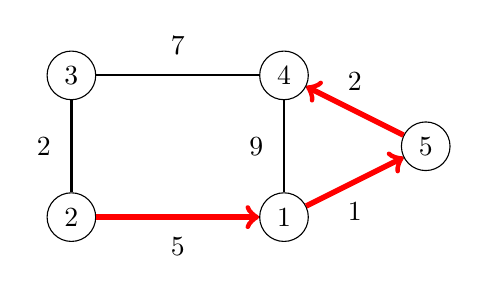
\begin{tikzpicture}[scale=0.9]
\node[draw, circle] (1) at (1,3) {$3$};
\node[draw, circle] (2) at (4,3) {$4$};
\node[draw, circle] (3) at (1,1) {$2$};
\node[draw, circle] (4) at (4,1) {$1$};
\node[draw, circle] (5) at (6,2) {$5$};

\path[draw,thick,-] (1) -- node[font=\small,label=above:7] {} (2);
\path[draw,thick,-] (1) -- node[font=\small,label=left:2] {} (3);
\path[draw,thick,-] (3) -- node[font=\small,label=below:5] {} (4);
\path[draw,thick,-] (2) -- node[font=\small,label=left:9] {} (4);
\path[draw,thick,-] (2) -- node[font=\small,label=above:2] {} (5);
\path[draw,thick,-] (4) -- node[font=\small,label=below:1] {} (5);

\path[draw=red,thick,->,line width=2pt] (3) -- (4);
\path[draw=red,thick,->,line width=2pt] (4) -- (5);
\path[draw=red,thick,->,line width=2pt] (5) -- (2);
\end{tikzpicture}
\end{center}

\subsubsection{Implementation}

The advantage of the
Floyd–Warshall algorithm that it is
easy to implement.
The following code constructs a
distance matrix where $\texttt{distance}[a][b]$
is the shortest distance between nodes $a$ and $b$.
First, the algorithm initializes \texttt{distance}
using the adjacency matrix \texttt{adj} of the graph:

\begin{lstlisting}
for (int i = 1; i <= n; i++) {
    for (int j = 1; j <= n; j++) {
        if (i == j) distance[i][j] = 0;
        else if (adj[i][j]) distance[i][j] = adj[i][j];
        else distance[i][j] = INF;
    }
}
\end{lstlisting}
After this, the shortest distances can be found as follows:
\begin{lstlisting}
for (int k = 1; k <= n; k++) {
    for (int i = 1; i <= n; i++) {
        for (int j = 1; j <= n; j++) {
            distance[i][j] = min(distance[i][j],
                                   distance[i][k]+distance[k][j]);
        }
    }
}
\end{lstlisting}

The time complexity of the algorithm is $O(n^3)$,
because it contains three nested loops
that go through the nodes of the graph.

Since the implementation of the Floyd–Warshall
algorithm is simple, the algorithm can be
a good choice even if it is only needed to find a
single shortest path in the graph.
However, the algorithm can only be used when the graph
is so small that a cubic time complexity is fast enough.
